\addcontentsline{toc}{chapter}{Занятие 2. Характеристики случайного процесса}
\chapter*{Занятие 2. Характеристики случайного процесса}

\addcontentsline{toc}{section}{Контрольные вопросы и задания}
\section*{Контрольные вопросы и задания}

\subsubsection*{Приведите определение случайного процесса.}

Случайный процесс $ \xi \left( t \right), \, t \in T$ ---
это параметризированная совокупность случайных величин.

\subsubsection*{Что называют конечномерными распределениями случайного процесса?}

$ \left\{ \mu_{t_1, \dotsc, t_n}; \, t_1, \dotsc, t_n \in T, \, n \geq 1 \right\} $ ---
набор конечномерных распределений процесса $ \xi $, где $ \mu_{t_1, \dotsc, t_n}$ ---
распределение вектора $ \left( \xi \left( t_1 \right), \dotsc, \xi \left( t_n \right) \right) $ в
$ \mathbb{R}^n$,
то есть для борелевского
$ \Delta \in \mathcal{B} \left( \mathbb{R}^n \right), \,
  \mu_{t_1, \dotsc, t_n} \left( \Delta \right) =
  P \left\{
    \left( \xi \left( t_1 \right), \dotsc, \xi \left( t_n \right) \right) \in \Delta
  \right\} $.

\subsubsection*{Приведите определение функции математического ожидания,
                дисперсии и ковариационной функции случайного процесса.}

$m \left( t \right) = M \xi \left( t \right), \, t \in T$ --- функция среднего.

$D \xi \left( t \right), \, t \in T$ --- функция дисперсии.

$K \left( t, s \right) =
  M \left[ \xi \left( t \right) - m \left( t \right) \right] \cdot
  \left[ \xi \left( s \right) - m \left( s \right) \right], \, t, s \in T$ ---
функция ковариации.

\addcontentsline{toc}{section}{Аудиторные задачи}
\section*{Аудиторные задачи}

\subsubsection*{2.2}

\textit{Задание.}
Пусть
$$ \xi \left( t \right) =
  X \cdot e^{-t}, \,
  t > 0,$$
где $X$ --- случайная величина,
которая имеет нормальное распределение с параметрами $a, \, \sigma^2$.
Найдите математическое ожидание, дисперсию,
ковариационную функцию и одномерную плотность распределения случайного процесса
$ \xi =
  \left\{ \xi \left( t \right), \, t > 0 \right\} $.

\textit{Решение.}
Сейчас $T = \left( 0, \infty \right) $.

Случайная величина $X$ имеет распределение $N \left( a, \sigma^2 \right) $.
Нужно найти $M \xi \left( t \right) = m \left( t \right), \, D \xi \left( t \right) $,
ковариационную функцию $K \left( t, s \right) $ и одномерную плотность распределения
$p_{ \xi } \left( t \right) $.

Найчнём с математического ожидания
$$m \left( t \right) =
  M \left( X \cdot e^{-t} \right) =
  e^{-t} MX =
  e^{-t} \cdot a.$$

Далее ---
функция дисперсии $D \xi \left( t \right) = D \left( X \cdot e^{-t} \right) = e^{-2t} \cdot DX$.
Дисперсия $X$ --- известная: $e^{-2t} \cdot DX = e^{-2t} \cdot \sigma^2$.

Далее ---
ковариационная функция
$$K \left( t, s \right) =
  M \left[ \xi \left( t \right) - m \left( t \right) \right] \cdot
  \left[ \xi \left( s \right) - m \left( s \right) \right] =
  cov \left[ \xi \left( t \right), \xi \left( s \right) \right].$$
Вместо $ \xi \left( t \right), \, \xi \left( s \right) $ подставляем их значения
$$cov \left[ \xi \left( t \right), \xi \left( s \right) \right] =
  cov \left( Xe^{-t}, Xe^{-s} \right).$$
Множители выносятся
$$cov \left( Xe^{-t}, Xe^{-s} \right) =
  e^{-t - s} cov \left( X, X \right) =
  e^{-t - s} DX =
  e^{-t - s} \sigma^2.$$

Последнее ---
это плотность $ \xi \left( t \right) \sim N \left( e^{-t} a, \, e^{-2t} \sigma^2 \right) $.

Нужно написать нормальную плотность с заданными математическим ожиданием и дисперсией
$$p_{ \xi \left( t \right) } \left( x \right) =
  \frac{1}{ \sqrt{2 \pi e^{-2t} \sigma^2}} \cdot
  e^{- \frac{ \left( x - e^{-t} a \right)^2}{2e^{-2t} \sigma^2}}.$$

Траектория процесса изображена на рисунке \ref{fig:22}
и имеет разный вид в зависимости от значения случайной величины $X$.

\begin{figure}[h!]
  \centering
  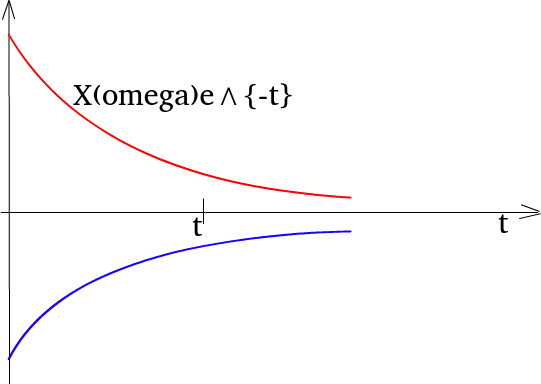
\includegraphics[width=.4\textwidth]{./pictures/2_2.png}
  \caption{Траектория процесса}
  \label{fig:22}
\end{figure}

\subsubsection*{2.3}

\textit{Задание.}
Пусть
$$ \xi \left( t \right) =
  e^{-Xt}, \,
  t > 0,$$
где $X$ --- случайная величина, которая имеет показательное распределение с параметром $ \lambda $.
Запишите конечномерные распределения случайного процесса
$ \left\{ \xi \left( t \right), \, t > 0 \right\} $.
Найдите его математическое ожидание, дисперсию и ковариационную функцию.

\textit{Решение.}
$ \xi \left( t \right) = e^{-Xt}$, где $X \sim Exp \left( \lambda \right), \, t > 0$.

Нужно найти $m \left( t \right), \, K \left( t, s \right) $, конечномерные распределения.

Найдём математическое ожидание в момент $t$.
По определению
$$m \left( t \right) =
  Me^{-Xt} =
  \int \limits_0^{+ \infty } \lambda e^{- \lambda x} e^{-Xt} dX =
  \frac{ \lambda }{ \lambda + t}.$$
Траектории такого процесса изображены на рисунке \ref{fig:23}: чем больше $X$,
тем быстрее эта функция убывает.

\begin{figure}[h!]
  \centering
  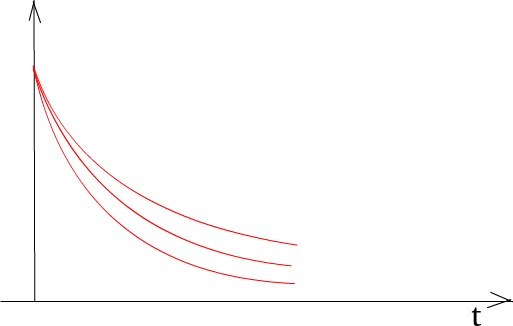
\includegraphics[width=.4\textwidth]{./pictures/2_3.png}
  \caption{Траектория процесса}
  \label{fig:23}
\end{figure}

Ковариационная функция считается по определению
$$K \left( t, s \right) =
  M \xi \left( t \right) \xi \left( s \right) - M \xi \left( t \right) M \xi \left( s \right) =
  Me^{-Xt - Xs} - \frac{ \lambda }{ \lambda + t} \cdot \frac{ \lambda }{ \lambda + s}.$$
Подставим найденное значение фунцкии математического ожидания
$$Me^{-Xt - Xs} - \frac{ \lambda }{ \lambda + t} \cdot \frac{ \lambda }{ \lambda + s} =
  \frac{ \lambda }{ \lambda + t + s} -
  \frac{ \lambda^2}{ \left( \lambda + t \right) \left( \lambda + s \right) }.$$

Считаем функцию распределения случайного вектора
$ \left( \xi \left( t_1 \right), \dotsc, \xi \left( t_n \right) \right) $ --- рис. \ref{fig:231}.

\begin{figure}[h!]
  \centering
  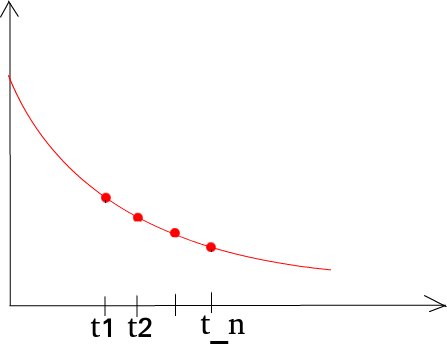
\includegraphics[width=.4\textwidth]{./pictures/2_3_1.png}
  \caption{Выбираем точки, в которых ищем распределение случайного процесса}
  \label{fig:231}
\end{figure}

$F_{ \left( \xi \left( t_1 \right), \dotsc, \xi \left( t_n \right) \right) }
  \left( \vec{x} \right) =
  P \left\{ \xi \left( t_1 \right) \leq x_1, \dotsc, \xi \left( t_n \right) \leq x_n \right\} $.
Вместо $ \xi $ напишем формулу
$P \left\{ \xi \left( t_1 \right) \leq x_1, \dotsc, \xi \left( t_n \right) \leq x_n \right\} =
  P \left( e^{-Xt_1} \leq x_1, \dotsc, e^{-Xt_n} \leq x_n \right) $.
Величины зависимы, потому что все они выражаются через $X$.
Все неравенства решаем относительно $X$
$$P \left( e^{-Xt_1} \leq x_1, \dotsc, e^{-Xt_n} \leq x_n \right) =
  P \left\{ X \geq -\frac{ln \, x_1}{t_1}, \dotsc, X \geq -\frac{ln \, x_n}{t_n} \right\}.$$
Перепишем через максимум
$$P \left\{ X \geq -\frac{ln \, x_1}{t_1}, \dotsc, X \geq -\frac{ln \, x_n}{t_n} \right\} =
  P \left\{
    X \geq \max \left( -\frac{ln \, x_1}{t_1}, \dotsc, -\frac{ln \, x_n}{t_n} \right) \right\}.$$
Обозначим максимум буквой $m$
$$P \left\{
    x \geq \max \left( -\frac{ln \, x_1}{t_1}, \dotsc, -\frac{ln \, x_n}{t_n} \right) \right\} =
  \int \limits_m^{+\infty } \lambda e^{-\lambda X} dX =
  -\left. e^{-\lambda X} \right|_m^{+\infty}.$$
На бесконечности получаем ноль
$$-\left. e^{-\lambda X} \right|_m^{+\infty} =
  e^{-\lambda m} =
  e^{-\lambda \max \left( ln \, x_1^{-\frac{1}{t_1}}, \dotsc, ln \, x_n^{-\frac{1}{t_n}} \right) }.$$
Выносим логарифм
$$e^{-\lambda \max \left( ln \, x_1^{-\frac{1}{t_1}}, \dotsc, ln \, x_n^{-\frac{1}{t_n}} \right) } =
e^{-\lambda ln \max \left( x_1^{-\frac{1}{t_1}}, \dotsc, x_n^{-\frac{1}{t_n}} \right) }.$$
Экспонента и логарифм уничтожают друг друга
$$e^{-\lambda ln \max \left( x_1^{-\frac{1}{t_1}}, \dotsc, x_n^{-\frac{1}{t_n}} \right) } =
  \max \left( x_1^{-\frac{1}{t_1}}, \dotsc, x_n^{-\frac{1}{t_n}} \right)^{-\lambda } =
  \min \left( x_1^{ \frac{ \lambda }{t_1}}, \dotsc, x_n^{ \frac{ \lambda }{t_n}} \right).$$

Все выкладки были законные, только когда $0 < x_1, \dotsc, x_n < 1$.

Плотности у такого векора $ \left( \xi \left( t_1 \right), \dotsc, \xi \left( t_n \right) \right) $
быть не может, потому что
$ \xi \left( t_1 \right)^{ \frac{1}{t_1}} =
  e^{-X} =
  \xi \left( t_2 \right)^{ \frac{1}{t_2}}$.
Сейчас у нас только одна случайная величина.
Это можно переписать как
$ \xi \left( t_2 \right) = \xi \left( t_1 \right)^{ \frac{t_2}{t_1}}, \,
  y = x^{ \frac{t_2}{t_1}}.$

С вероятностью 1 $ \left( \xi \left( t_1 \right), \xi \left( t_2 \right) \right) \in L$ ---
рис. \ref{fig:232}.

\begin{figure}[h!]
  \centering
  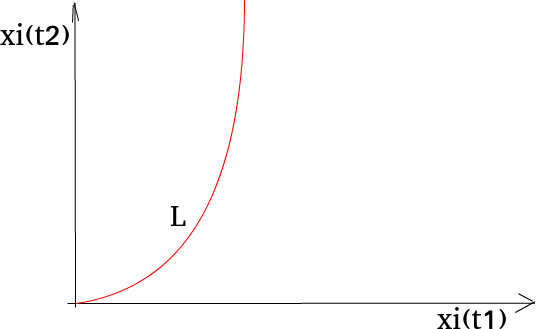
\includegraphics[width=.4\textwidth]{./pictures/2_3_2.png}
  \caption{$y = x^{ \frac{t_2}{t_1}}$}
  \label{fig:232}
\end{figure}

Значения вектора всегда попадают на такую линию.
Площадь кривой --- ноль.

Плотность --- производная от функции распределения, а минимум нельзя дифференцировать.

\addcontentsline{toc}{section}{Домашнее задание}
\section*{Домашнее задание}
